% !TEX TS-program = pdflatex
% !TEX encoding = UTF-8 Unicode

% This is a simple template for a LaTeX document using the "article" class.
% See "book", "report", "letter" for other types of document.

\documentclass[20pt]{article} % use larger type; default would be 10pt

\usepackage[utf8]{inputenc} % set input encoding (not needed with XeLaTeX)

%%% Examples of Article customizations
% These packages are optional, depending whether you want the features they provide.
% See the LaTeX Companion or other references for full information.

%%% PAGE DIMENSIONS
\usepackage{geometry} % to change the page dimensions
\geometry{a4paper} % or letterpaper (US) or a5paper or....
% \geometry{margin=2in} % for example, change the margins to 2 inches all round
% \geometry{landscape} % set up the page for landscape
%   read geometry.pdf for detailed page layout information

\usepackage{graphicx} % support the \includegraphics command and options

% \usepackage[parfill]{parskip} % Activate to begin paragraphs with an empty line rather than an indent

%%% PACKAGES
\usepackage{booktabs} % for much better looking tables
\usepackage{array} % for better arrays (eg matrices) in maths
\usepackage{paralist} % very flexible & customisable lists (eg. enumerate/itemize, etc.)
\usepackage{verbatim} % adds environment for commenting out blocks of text & for better verbatim
%\usepackage{subfig} % make it possible to include more than one captioned figure/table in a single float
\usepackage{mathtools}
\usepackage{graphicx} % supports images in latex
% These packages are all incorporated in the memoir class to one degree or another...

\usepackage{graphicx}
\usepackage{subcaption}

%%% Other stuff
\DeclarePairedDelimiter\ceil{\lceil}{\rceil}
\DeclarePairedDelimiter\floor{\lfloor}{\rfloor}

%%% HEADERS & FOOTERS
\usepackage{fancyhdr} % This should be set AFTER setting up the page geometry
\pagestyle{fancy} % options: empty , plain , fancy
\renewcommand{\headrulewidth}{0pt} % customise the layout...
\lhead{}\chead{}\rhead{}
\lfoot{}\cfoot{\thepage}\rfoot{}

%%% SECTION TITLE APPEARANCE
\usepackage{sectsty}
\allsectionsfont{\sffamily\mdseries\upshape} % (See the fntguide.pdf for font help)
% (This matches ConTeXt defaults)

%%% ToC (table of contents) APPEARANCE
\usepackage[nottoc,notlof,notlot]{tocbibind} % Put the bibliography in the ToC
\usepackage[titles,subfigure]{tocloft} % Alter the style of the Table of Contents
\renewcommand{\cftsecfont}{\rmfamily\mdseries\upshape}
\renewcommand{\cftsecpagefont}{\rmfamily\mdseries\upshape} % No bold!

%%% graphics path


%%% END Article customizations

%%% nice things to keep around
%\begin{figure}[!htbp]
%  	\centering
%   	\begin{subfigure}[p]{0.5\linewidth}
%    	\includegraphics[width=\linewidth]{}
%   	\end{subfigure}
%\end{figure} 

% \noindent\rule{2cm}{0.4pt} 
%%% puts a small horizontal line

% \mathcal{O} 
%%% big O notation

% \begin{table}
% \caption{Forward slash.}
% \[\begin{array}{c|ccccc} 
% abc/def & 1 & 2 & 3 & 4 & 5\\
% \hline
% 1 & a & b & c & d & e\\
% 2 & f & g & h & i & j\\
% 3 & k & l & m & n & o\\
% \end{array}\]
% \end{table}

%%% The "real" document content comes below...

\title{Formal Languages Homework 4}
\author{Liam Dillingham}
%\date{} % Activate to display a given date or no date (if empty),
         % otherwise the current date is printed 

\begin{document}
\maketitle

\section{Problem 3.2.2}
Here is a transition table for a DFA:
\begin{figure}[!htbp]
  	\centering
   	\begin{subfigure}[p]{0.25\linewidth}
    	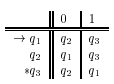
\includegraphics[width=\linewidth]{./figures/HW4fig1.png}
   	\end{subfigure}
\end{figure} 

% NOTE: For all answers to this question, I'm relabeling all states $q_i$ to their index, $i$.

\subsection{a) Give all the regular expressions $R_{ij}^{(0)}$. Note: Think of state $q_i$ as if it were the state with integer number $i$.}

\begin{table}[!htbp]
% \caption{Forward slash.}
\[\begin{array}{c|ccc}
R_{ij}^{(0)} & q_1 & q_2 & q_3 \\
\hline
\rightarrow q_1 & \epsilon & 0 & 1 \\
q_2 & 0 & \epsilon & 1 \\
^{*}q_3 & 1 & 0 & \epsilon \\
\end{array}\]
\end{table}

\subsection{b) Give all the regular expressions $R_{ij}^{(1)}$. Try to simplify the expressions as much as possible}
$R_{ij}^{(1)} = R_{ij}^{(0)} + R_{i1}^{(0)}(R_{11}^{(0)})^{*}R_{1j}^{(0)}$
\begin{table}[!htbp]
% \caption{Forward slash.}
\[\begin{array}{c|ccc}
R_{ij}^{(1)} & q_1 & q_2 & q_3 \\
\hline
\rightarrow q_1 & \epsilon & 0 & 1 \\
q_2 & 0 & \epsilon + 00 & 1+01 \\
^{*}q_3 & 1 & 0+00 & \epsilon+1 \\
\end{array}\]
\end{table}

\newpage
\subsection{c) Give all the regular expressions $R_{ij}^{(2)}$. Try to simplify the expressions as much as possible}
$R_{ij}^{(2)} = R_{ij}^{(1)} + R_{i2}^{(1)}(R_{22}^{(1)})^{*}R_{2j}^{(1)}$
\begin{table}[!htbp]
% \caption{Forward slash.}
\[\begin{array}{c|ccc}
R_{ij}^{(1)} & q_1 & q_2 & q_3 \\
\hline
\rightarrow q_1 & \epsilon+0(\epsilon+00)^{*}0 & 0+0(\epsilon+00)^{*}(\epsilon+00) & 1+0(\epsilon+00)^{*}(1+01) \\
q_2 & 0+(\epsilon+00)(\epsilon+00)^{*}0 & \epsilon+00+(\epsilon+00)(\epsilon+00)^{*}(\epsilon+00) & 1+01+(\epsilon+00)(\epsilon+00)^{*}(1+01) \\
^{*}q_3 & \epsilon+1+(0+00)(\epsilon+00)^{*}0 & 0+00+(0+00)(\epsilon+00)^{*}(\epsilon+00) & \epsilon+1+(0+00)(\epsilon+00)^{*}(1+01) \\
\end{array}\]
\end{table}

\subsection{d) Give a regular expression for the language of the automaton}

final answer: $1+0(00)^{*}(01+0)((10+1)(00)^{*}(01+0)+11)^{*}$.

\newpage
\section{Problem 3.2.3}
Convert the following DFA to a regular expression, using the state-elimination technique of Section 3.2.2 
\begin{figure}[!htbp]
  	\centering
   	\begin{subfigure}[p]{0.2\linewidth}
    	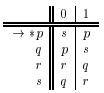
\includegraphics[width=\linewidth]{./figures/HW4fig2.png}
   	\end{subfigure}
\end{figure} \\
\noindent\rule{2cm}{0.4pt} \\

I wanted to include the scratchwork I used to calculate the regular expression:
\begin{figure}[!htbp]
  	\centering
   	\begin{subfigure}[p]{0.6\linewidth}
    	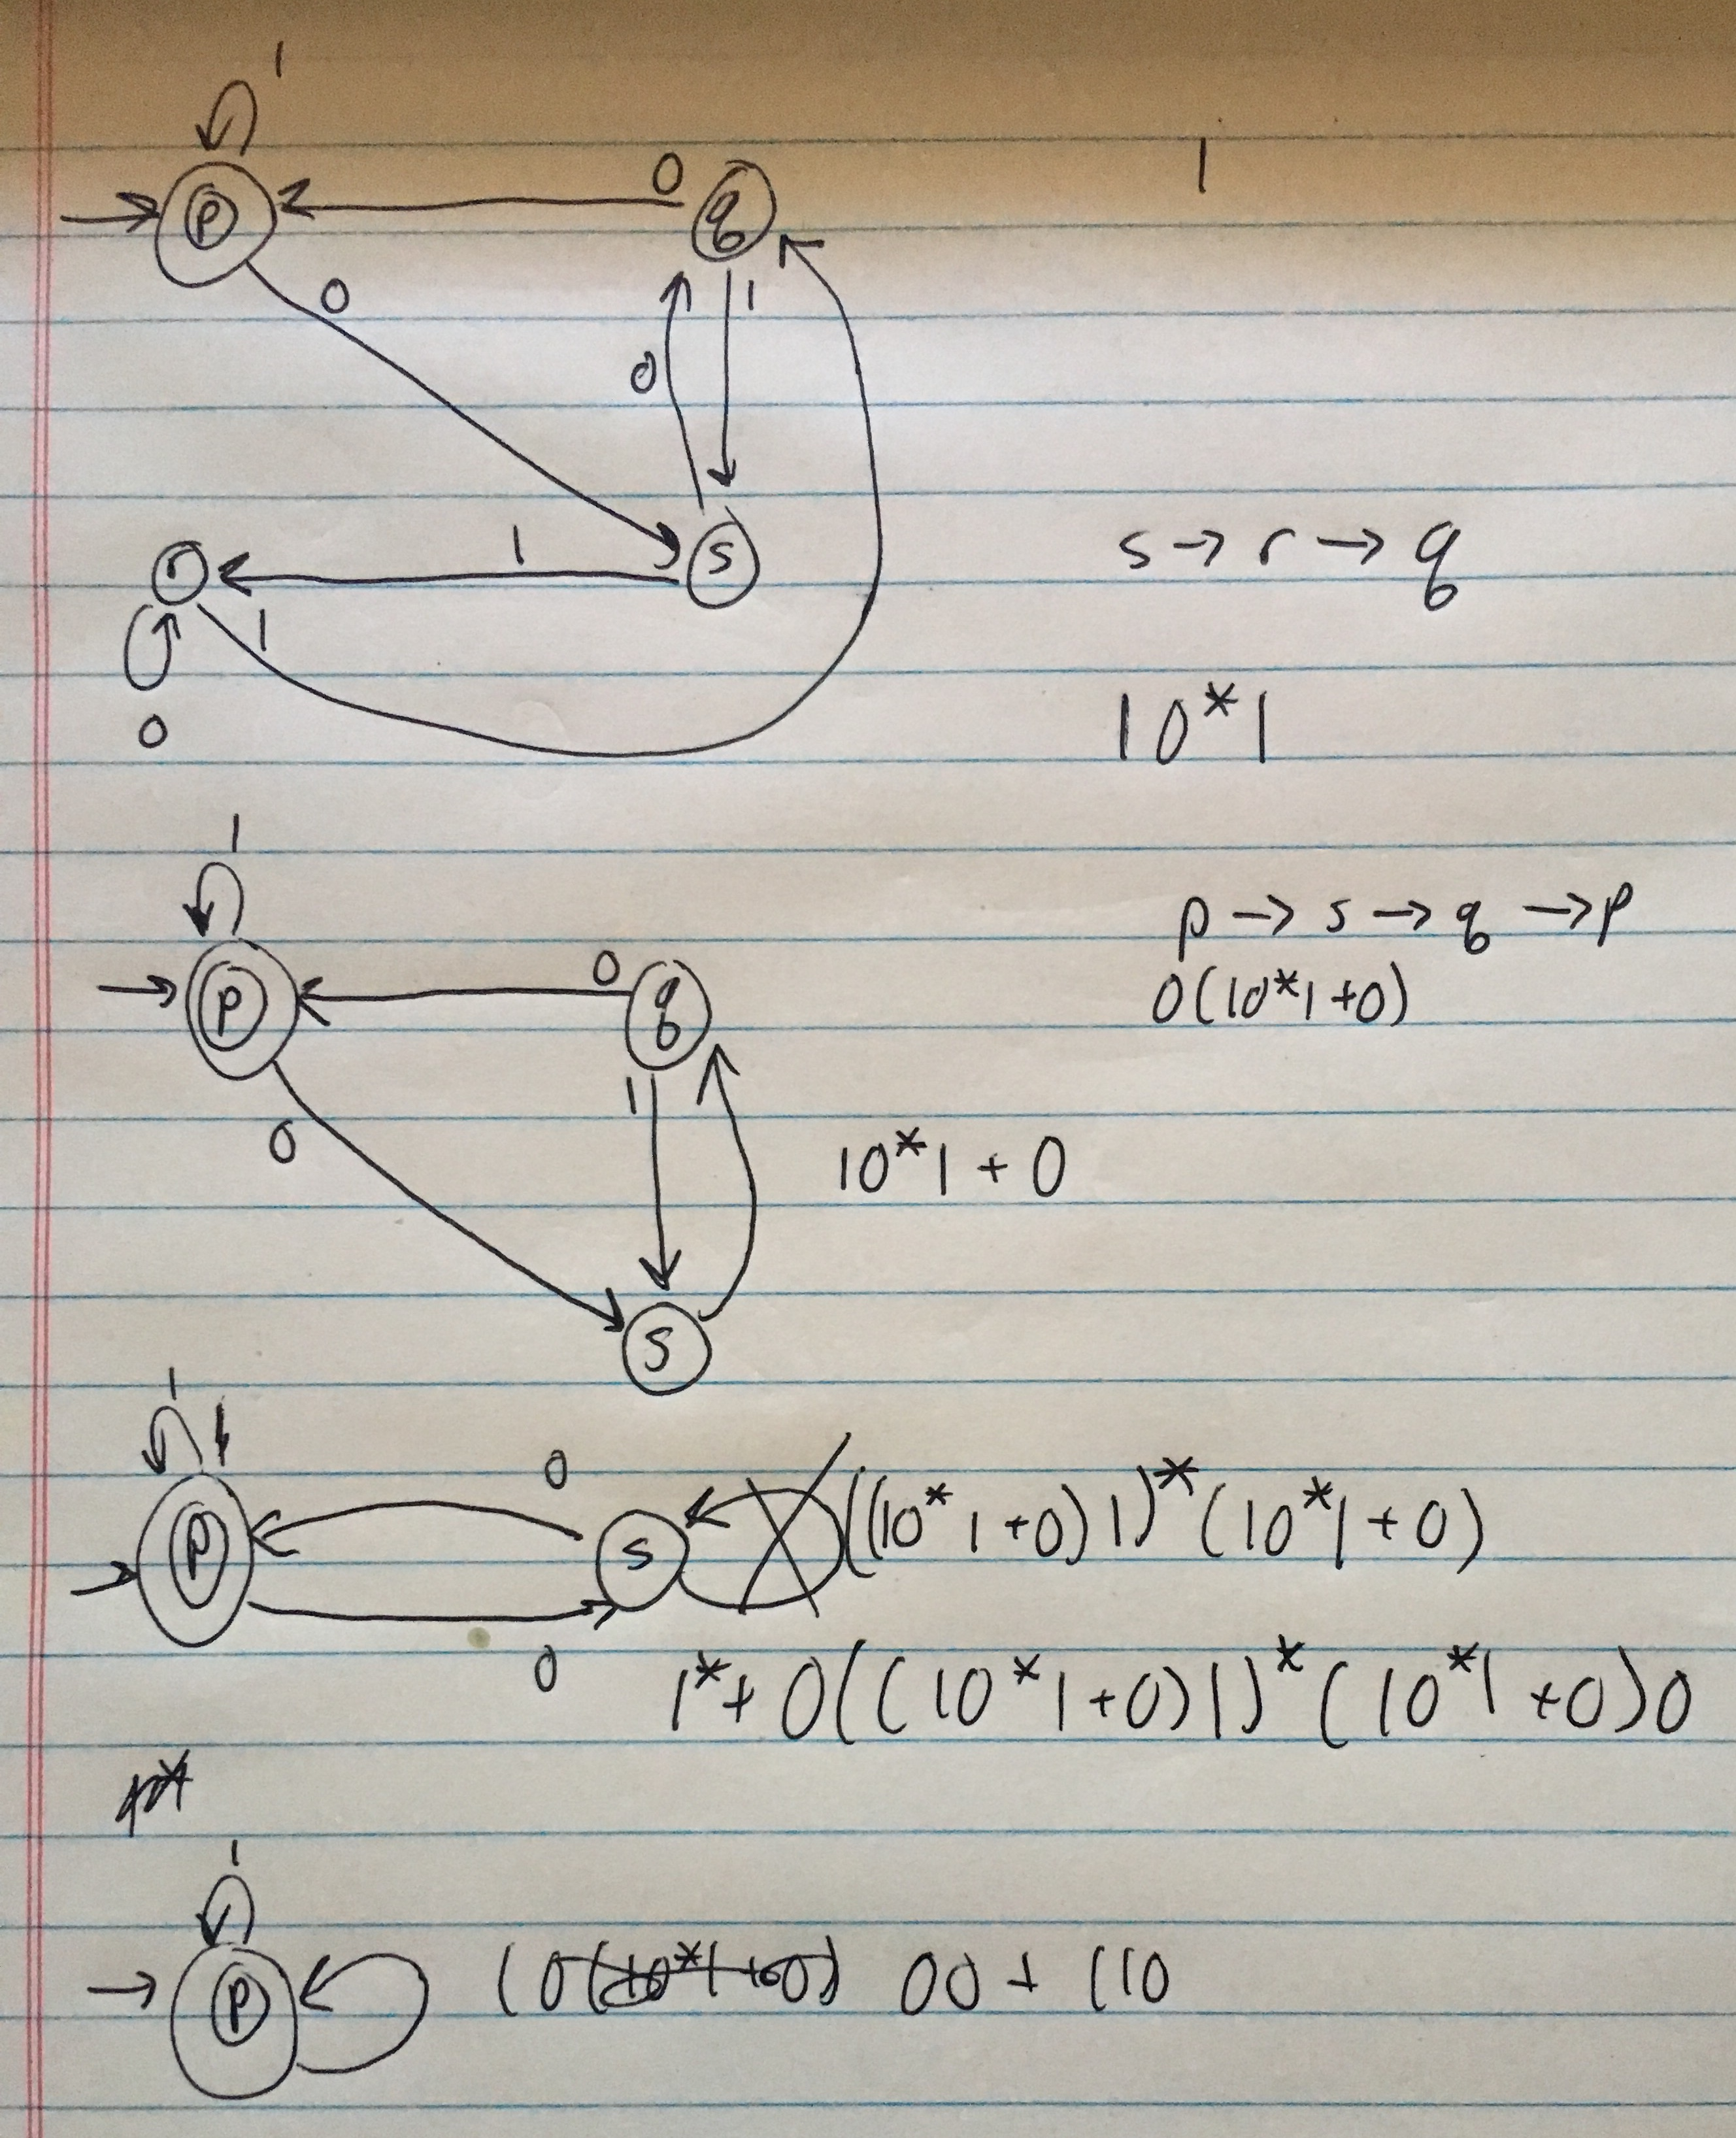
\includegraphics[width=\linewidth]{./figures/h4-1.jpg}
   	\end{subfigure}
\end{figure} \\
Final Answer: \\ 
$1^{*}+(0(1+10^{*}1)(0(1+10^{*}1))^{*}0$

\newpage
\section{Problem 3.2.4}
Convert the following regular expressions to NFA's with $\epsilon$-transitions.
\subsection{b) $(0+1)01$}
\begin{figure}[!htbp]
  	\centering
   	\begin{subfigure}[p]{0.8\linewidth}
    	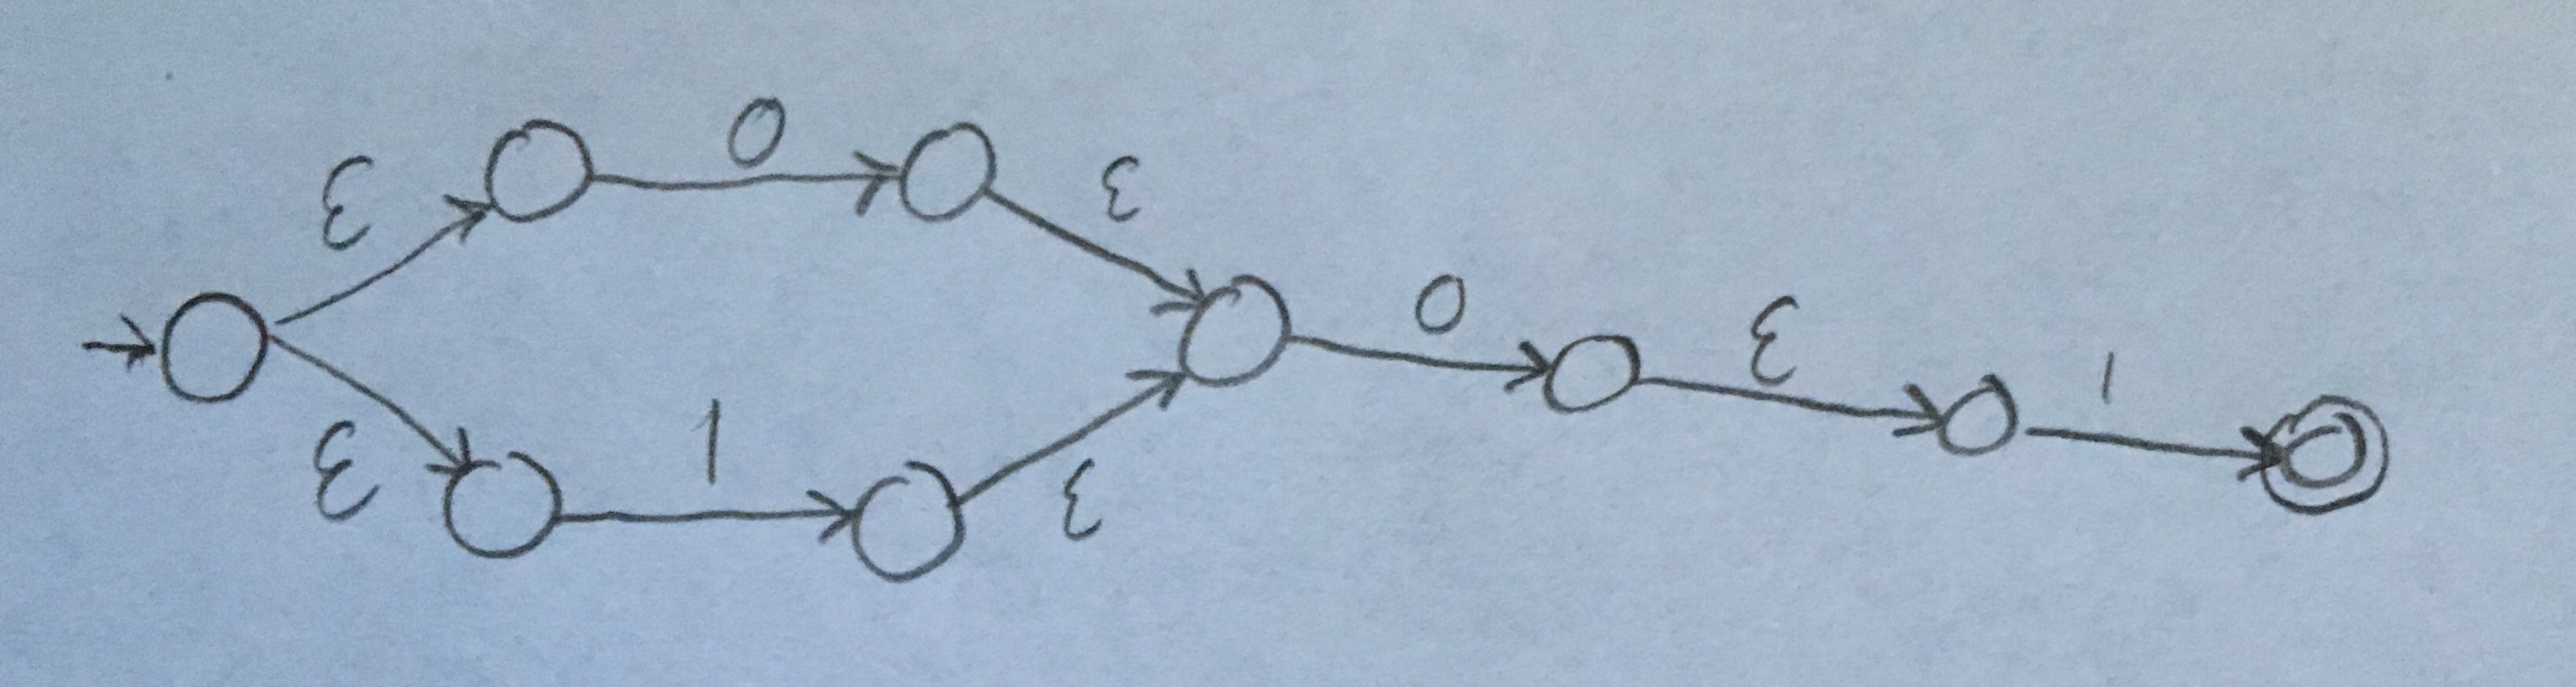
\includegraphics[width=\linewidth]{./figures/h4-2.jpg}
   	\end{subfigure}
\end{figure}
\subsection{c) $00(0+1)^{*}$}
\begin{figure}[!htbp]
  	\centering
   	\begin{subfigure}[p]{0.8\linewidth}
    	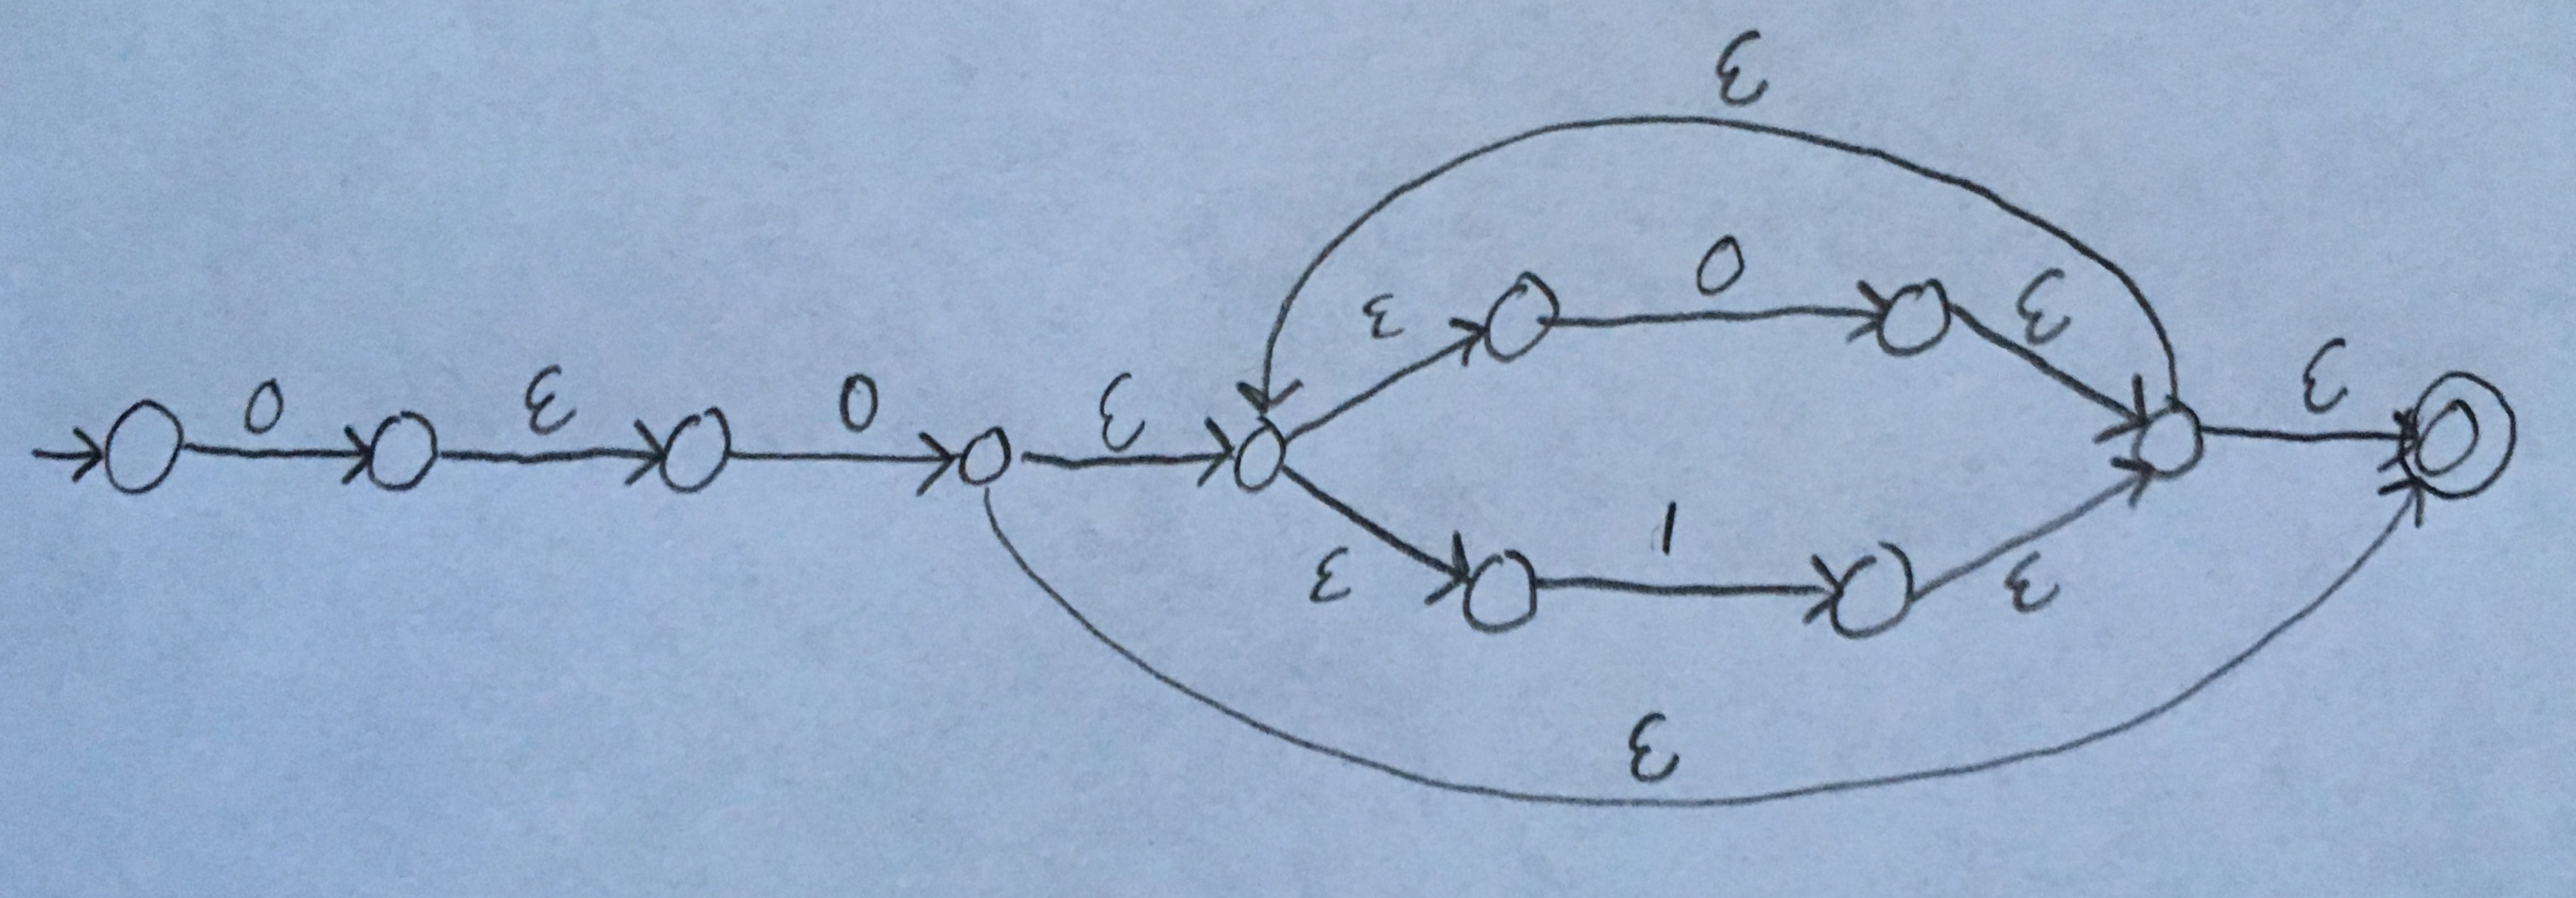
\includegraphics[width=\linewidth]{./figures/h4-3.jpg}
   	\end{subfigure}
\end{figure}

\newpage
\section{Problem 3.4.1}
Verify the following identities involving regular expressions.
\subsection{b) $(R+S)+T=R+(S+T)$}

Let $r \in R, s \in S, t \in T$ be representative elements from their respective regular expressions. Starting on the left hand side, we have $r+s = \{r,s\}$. Then $\{r,s\}+t = \{r,s,t\}$. For the right hand side, we have $s+t = \{s,t\}$, and then $r+\{s,t\}=\{r,s,t\}$. Thus the two sides are equal.

\subsection{c) $(RS)T=R(ST)$}
Let $r \in R, s \in S, t \in T$ be representative elements from their respective regular expressions. $rs$ produces the set $\{rs\}$, with $t$ gives us $\{rst\}$.  Similarly, $st$ gives us $\{st\}$, and with $r$ we have $\{rst\}$.  Both sides are equal.

\subsection{h) $(R^{*}S^{*})^{*}=(R+S)^{*}$}
Let $r \in R, s \in S$ be representative elements from their respective regular expressions.  Note on the right hand side, we have the set $\{r,s\}$.  Then to compute the kleene closure, we pick an element from this set and append it to our word.  We get a set like this: $\{\epsilon, r, s, rs, sr, ssr, rrs, srs, rsr, rrr, ..\}$. That is, every combination of $s$'s and $r$'s for any length. For the right hand side, we have $R^{*} = \{\epsilon, r, rr, rrr, ...\}$, and $S^{*} = \{\epsilon, s, ss, sss, ...\}$. Then we compute the closure of the concatenation of these two sets. Then we dot these two sets together, giving us a set with an arbitrary number of $r$'s on the left, and $s$'s on the right.  With this, we compute the kleene closure, where we pick an arbitrary number of elements from our set and concatenate them.  To prove this simply, note that both $r$ and $s$ are in this set, that is $\{r,s\} \subset R^{*}S^{*}$. Then, by simply selecting from this small subset, we can build a string of arbitrary length of any combination of $s$'s and $r$'s.  Thus, the two sets are equal.


\end{document}






